\subsubsection{\texorpdfstring{$\Ph\to\Pa\Pa\to\PGm\PGm\PGm\PGm$}{Higgs to two a to mu mu mu mu }}
\label{subsec:fourmu}

\begin{center}
 {Alfredo Castaneda$^{1}$, Sven Dildick$^{2}$, Luca Pernie$^{2}$ and Jamal Rorie$^{3}$ \\
}
\centerline{{\it  $^{1}$Department of Physics and Astronomy, University of Sonora, Mexico}}
\centerline{{\it $^{2}$Department of Physics and Astronomy, Texas A\&M University, USA}}
\centerline{{\it  $^{3}$Department of Physics and Astronomy, Rice University, USA}}
\end{center}

\ifthenelse{\boolean{cms@external}}{\setlength\cmsFigWidth{0.49\textwidth}}{\setlength\cmsFigWidth{0.65\textwidth}} % example: one column in journal, 2/3 in CMS
\ifthenelse{\boolean{cms@external}}{\providecommand{\cmsLeft}{upper\xspace}}{\providecommand{\cmsLeft}{left\xspace}}
\ifthenelse{\boolean{cms@external}}{\providecommand{\cmsRight}{lower\xspace}}{\providecommand{\cmsRight}{right\xspace}}
\newcommand{\processbbtt}{\ensuremath{{\Ph}\to{\Pa\Pa}\to2\Pgt2{\cPqb}}\xspace}
\newcommand{\processmmtt}{\ensuremath{{\Ph}\to{\Pa\Pa}\to2\Pgm2{\Pgt}}\xspace}
\newcommand{\ma}{\ensuremath{m_{\Pa}}\xspace}
\newcommand{\mbtt}{\ensuremath{m_{\cPqb\Pgt\Pgt}^{\text{vis}}}\xspace}

% quick test

% Spectator particles
\newcommand{\PX}{\ensuremath{\mathrm{X}}\xspace}
% Dark Photon
\newcommand{\gammaDark}{\ensuremath{{\PGg}_{\mathrm{D}}}\xspace}
% Visible Neutralino (n_1)
\newcommand{\nOne}{\ensuremath{\textnormal{n}_{1}}\xspace}
% Dark Neutralino
\newcommand{\nDark}{\ensuremath{\textnormal{n}_{\mathrm{D}}}\xspace}
% CP-even NMSSM Higgs One
\newcommand{\PhOne}{\ensuremath{\Ph_{1}}\xspace}
% CP-even NMSSM Higgs Two
\newcommand{\PhTwo}{\ensuremath{\Ph_{2}}\xspace}
% CP-even NMSSM Higgs One,Two
\newcommand{\PhOneTwo}{\ensuremath{\Ph_{1,2}}\xspace}
% CP-odd NMSSM Higgs One
\newcommand{\PaOne}{\ensuremath{\Pa_{1}}\xspace}
% Dimuon
\newcommand{\dimuon}{\ensuremath{(\PGm\PGm)}\xspace}
% DimuonOne
\newcommand{\dimuonOne}{\ensuremath{(\PGm\PGm)_1}\xspace}
% DimuonTwo
\newcommand{\dimuonTwo}{\ensuremath{(\PGm\PGm)_2}\xspace}

% Mass of Dark Photon
\newcommand{\MgammaDark}{\ensuremath{m_{{\PGg}_{\mathrm{D}}}}\xspace}
% Mass of Visible Neutralino (n_1)
\newcommand{\MnOne}{\ensuremath{m_{{\textnormal{n}}_{1}}}\xspace}
% Mass of Dark Neutralino
\newcommand{\MnDark}{\ensuremath{m_{{\textnormal{n}}_{\mathrm{D}}}}\xspace}
% Mass of CP-even NMSSM Higgs One
\newcommand{\MPhOne}{\ensuremath{m_{\Ph_{1}}}\xspace}
% Mass of CP-even NMSSM Higgs Two
\newcommand{\MPhTwo}{\ensuremath{m_{\Ph_{2}}}\xspace}
% Mass of CP-even NMSSM Higgs Two
\newcommand{\MPhOneTwo}{\ensuremath{m_{\Ph_{1,2}}}\xspace}
% Mass of CP-even NMSSM Higgs i
\newcommand{\MPhI}{\ensuremath{m_{\Ph_{i}}}\xspace}
% Mass of CP-odd NMSSM Higgs (generic)
\newcommand{\MPa}{\ensuremath{m_{\Pa}}\xspace}
% Mass of CP-odd NMSSM Higgs a1
\newcommand{\MPaOne}{\ensuremath{m_{\Pa_{1}}}\xspace}
% Mass of Dimuon (Generic)
\newcommand{\Mdimuon}{\ensuremath{m_{(\PGm\PGm)}}\xspace}
% Mass of Dimuon One
\newcommand{\MdimuonOne}{\ensuremath{m_{(\PGm\PGm)_1}}\xspace}
% Mass of Dimuon Two
\newcommand{\MdimuonTwo}{\ensuremath{m_{(\PGm\PGm)_2}}\xspace}
% Mass of the muon
\newcommand{\Mmuon}{\ensuremath{m_{\PGm}}\xspace}
% Mass of the tau

% Lifetime of Dark Photon
\newcommand{\TgammaDark}{\ensuremath{\tau_{{\PGg}_{\mathrm{D}}}}\xspace}


% Ratio parameter (r)
\newcommand{\ratio}{\ensuremath{\overline{r}}\xspace}
% Alpha Gen
\newcommand{\alphaGen}{\ensuremath{\alpha_\text{gen}}\xspace}
% Epsilon Full
\newcommand{\epsilonFull}{\ensuremath{\varepsilon_{\text{full}}}\xspace}
% S Template I
\newcommand{\SOne}{\ensuremath{S_\mathrm{I}(\Mdimuon)}\xspace}
% S Template II
\newcommand{\STwo}{\ensuremath{S_\mathrm{II}(\Mdimuon)}\xspace}
% Diagonal Area (Signal Region)
\newcommand{\ASR}{\ensuremath{A_{\mathrm{SR}}}\xspace}
% Off-Diagonal Area (Control Region)
\newcommand{\ACR}{\ensuremath{A_{\mathrm{CR}}}\xspace}
% Fraction SPS
\newcommand{\fSPS}{\ensuremath{f_\mathrm{SPS}}\xspace}

In this analysis, the search for a new light boson is focused on events where four final-state muons reconstruct to a pair of dimuons~\cite{CMS-PAS-HIG-18-003}. These dimuons must have a common decay vertex and a similar invariant mass. The dimuon mass is allowed to vary between between 0.25 and 8.5\GeV; their lifetimes can range up to $c\tau=100\mm$. Standard model backgrounds are reduced due to the dimuon vertex constraint and mass criteria as well as isolation requirements on the constituent muons. To avoid the introduction of bias between models in the trigger, we require the presence of a ``high $p_\mathrm{T}$'' muon: a muon with with $p_\mathrm{T} > 17\GeV$ located in the barrel region. The criteria are examined in the context of multiple models to ensure that there is no model sensitivity. The remaining background is sparse and is dominated by decays of \bbbar quarks, with small-to-negligible contributions from promptly produced \JPsi mesons and electroweak processes. This background is modeled with a two-dimensional template as a function of dimuon mass. The \bbbar contribution to the background template, normalized to unity, is shown in Fig.~\ref{fig:2dtemplate}. Since the width of the new particle is expected to be extremely narrow, the signal shape for each mass point is modeled according to a Crystal Ball \cite{Oreglia:1980cs} function for which the width is solely determined by the resolution of the muon system. The template is used along with any observed events to extract a limit as part of modified frequentist procedure. This result can then be interpreted in the context of specific models.

\begin{figure}[tb]
\begin{center}
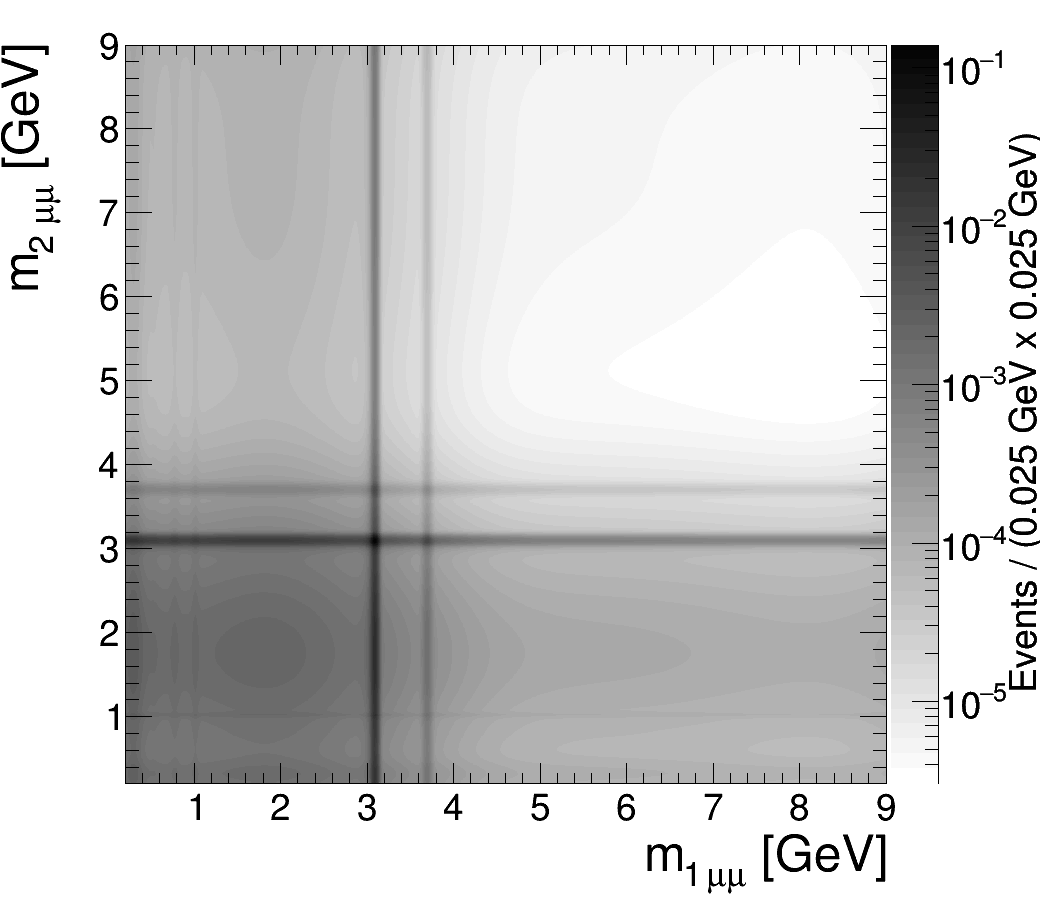
\includegraphics[width=0.52\linewidth]{plots/h2_background.png}
\end{center}
\caption{The 2D analytical template for distribution of the dimuon masses obtained using background-enriched data sample, normalized to unity. \label{fig:2dtemplate}}
\end{figure}

The projected CL upper limits on ${\sigma(\Pp\Pp \to 2 \Pa + \PX)  \mathcal{B}^2 (\Pa \to 2\PGm)  \alphaGen}$ for the $\Ph\to\Pa\Pa\to4\PGm$ analysis is shown in Fig.~\ref{fig:my_label1}. The upper limits scale approximately as the inverse of the integrated luminosity. The results are interpreted in the NMSSM in Fig.~\ref{fig:my_label2}, and in models with dark photons in Fig.~\ref{fig:my_label4}, for the scenario with YR18 systematic uncertainties and using 3000\fbinv. The results obtained using 3000\fbinv with run 2 systematic uncertainties were not found to be significantly different.

Compared to the results in Ref.~\cite{CMS-PAS-HIG-18-003} obtained with 36\fbinv, the limit on $\sigma \left( \Pp\Pp \to \PhOneTwo \to 2 \PaOne \right) \mathcal{B}^2(\PaOne \to 2\PGm)$ is approximately a factor 80 smaller with integrated luminosity of 3000\fbinv of data. In models with dark photons, more stringent limits were set on the kinetic mixing parameter $\varepsilon$. In addition, the search becomes more sensitive to models with BR = 0.1\% beyond the $\rho$ meson mass.

%% Divide up: Analysis techniques, then hardware improvements.
%% state briefly that the results are conservative
They should be considered as lower bounds of the sensitivity of this analysis. The analysis methods used in the search on Run 2 data from 2016 were neither reviewed nor optimized for this projection. The methods do not consider anticipated improvements to the analysis techniques nor the effect of upgrades to the LHC and CMS hardware. The results are thus extremely conservative estimates.

%% explain how the projection is dominated by background
This search is designed to have almost no background contribution. However, as this projection was made with non-optimized background modeling techniques, a non-trivial number of background events (primarily from bottom quark pair production, \bbbar) enter the search region when the integrated luminosity is 3000\fbinv. As such, the sensitivity is expected to be dominated by the background contribution in this simple projection. The systematic uncertainties have a negligible effect on the model independent upper limit on the product of the cross section, the branching fraction, and the acceptance. The limits for scenario 2 with smaller systematic uncertainties are not significantly better than for scenario 1.
%Do we want to consider the narrowing of the signal region?
%% extended mass range - briefly address difficulties in background modeling?

The search can also be extended to search for new bosons that are more massive. Searches could be performed for $\ma$ up to 62.5\GeV. Preliminary studies indicate that the modeling of the leading background, \bbbar, would have to be revised.
%% improved vertex finding, dimuon reconstruction, etc

%% explain how the results would be improved in Run-3 and Run-4
%This search may be improved considerably with the upgraded CMS detector at the HL-LHC.
This search may be improved considerably with the HL-LHC upgrade and upgrades to the CMS detector.
%% higher center of mass energy
The sensitivity to $\Ph\to\Pa\Pa\to\PGm\PGm\PGm\PGm$ events will increase as the center-of-mass energy increases from 13 to 14\TeV. The main production channel ggF will increase by as much as 12\% \cite{deFlorian:2016spz}. Additional Higgs boson production modes, associated production and ttbarH, will improve the sensitivity as well.
%https://twiki.cern.ch/twiki/bin/view/LHCPhysics/CERNYellowReportPageAt13TeV
%https://twiki.cern.ch/twiki/bin/view/LHCPhysics/CERNYellowReportPageAt14TeV
%% few words about the size of the search region in the dimuon-dimuon spectrum

%% new muon and tracker system
Data taking with an upgraded tracker and muon system may potentially have a dramatic effect on the fiducial search region.
%% eta and pt selection cuts
The commissioning of new GEM-based detectors in the forward region could extend the fiducial region from $|\eta| < 2.4$ to $|\eta| < 2.8$. In addition, the momentum assignment could improve significantly in the overlap and endcap region, so that high-pT dimuons may also be selected beyond $|\eta| > 0.9$.
%% Lxy cut

The transverse displacement of the new light boson decay vertex, $L_{xy}$, was limited to 9.8\cm in the search with the 2016 data set. By making use of new muon finding techniques optimized for displacement in the L1 trigger, the high level trigger, and in offline reconstruction, the range of transverse displacement in which a new light boson decay can be detected may increase to {1--3 m}. %The analysis would then sensitive to signatures with $c\tau=1000\mm$.
Such an increase in the range of $L_{xy}$ would correspond to an upper limit on the kinetic mixing parameter $\varepsilon$ as low as $\varepsilon<10^{-10}$.

Finally, the object reconstruction and selection should be revisted and optimized for signatures with dimuons in pp collision data at the HL-LHC.

\begin{figure}
\centering
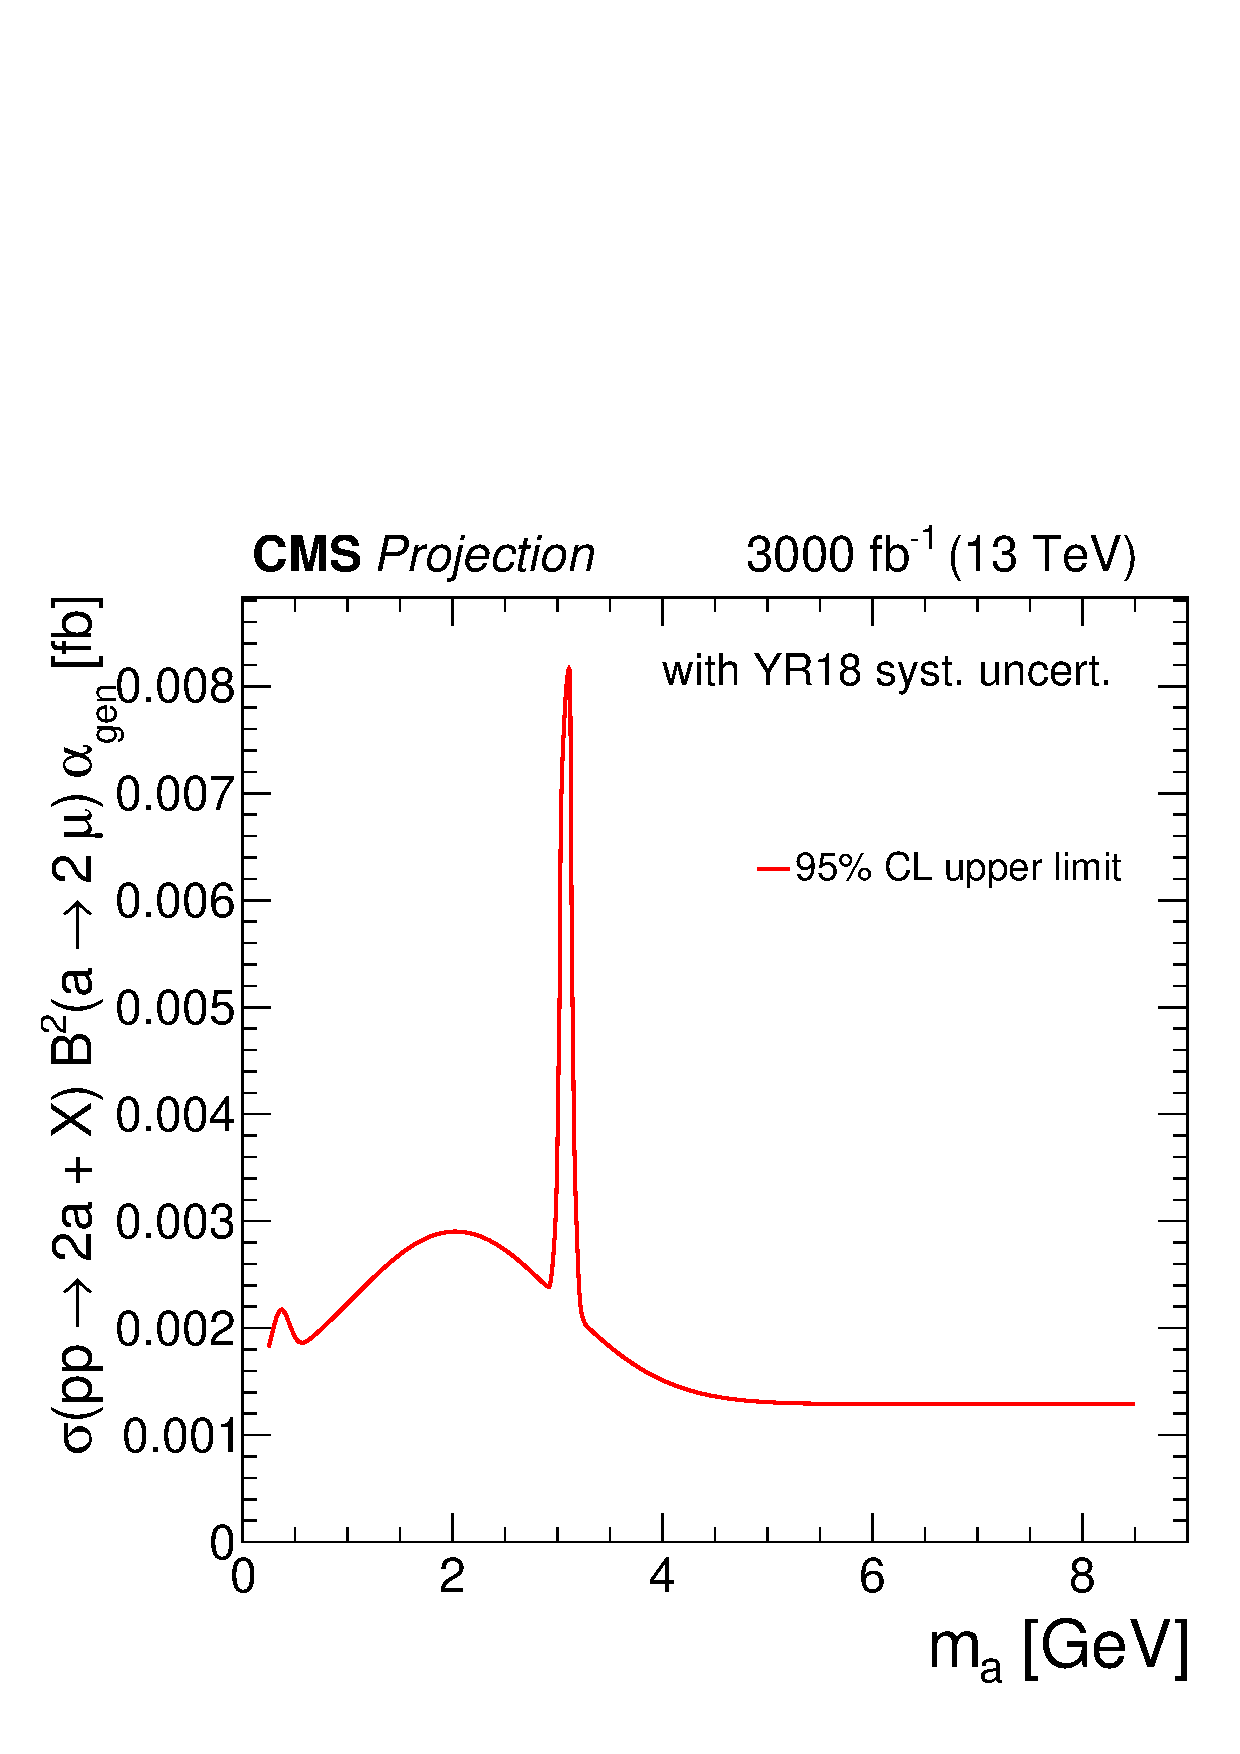
\includegraphics[width=0.47\textwidth]{plots/nmssm_plots_scenario_2/limit_CSxBR2xAlpha_fb_vs_mGammaD_3000.pdf}
\caption{Projected 95\% \CL upper limits on ${\sigma(\Pp\Pp \to 2 \Pa + \PX)  \mathcal{B}^2 (\Pa \to 2\PGm)  \alphaGen}$ over the range ${0.25 < \MPa < 8.5\GeV}$ for 3000\fbinv of data in the scenario with YR18 systematic uncertainties.}
\label{fig:my_label1}
\end{figure}

\begin{figure}
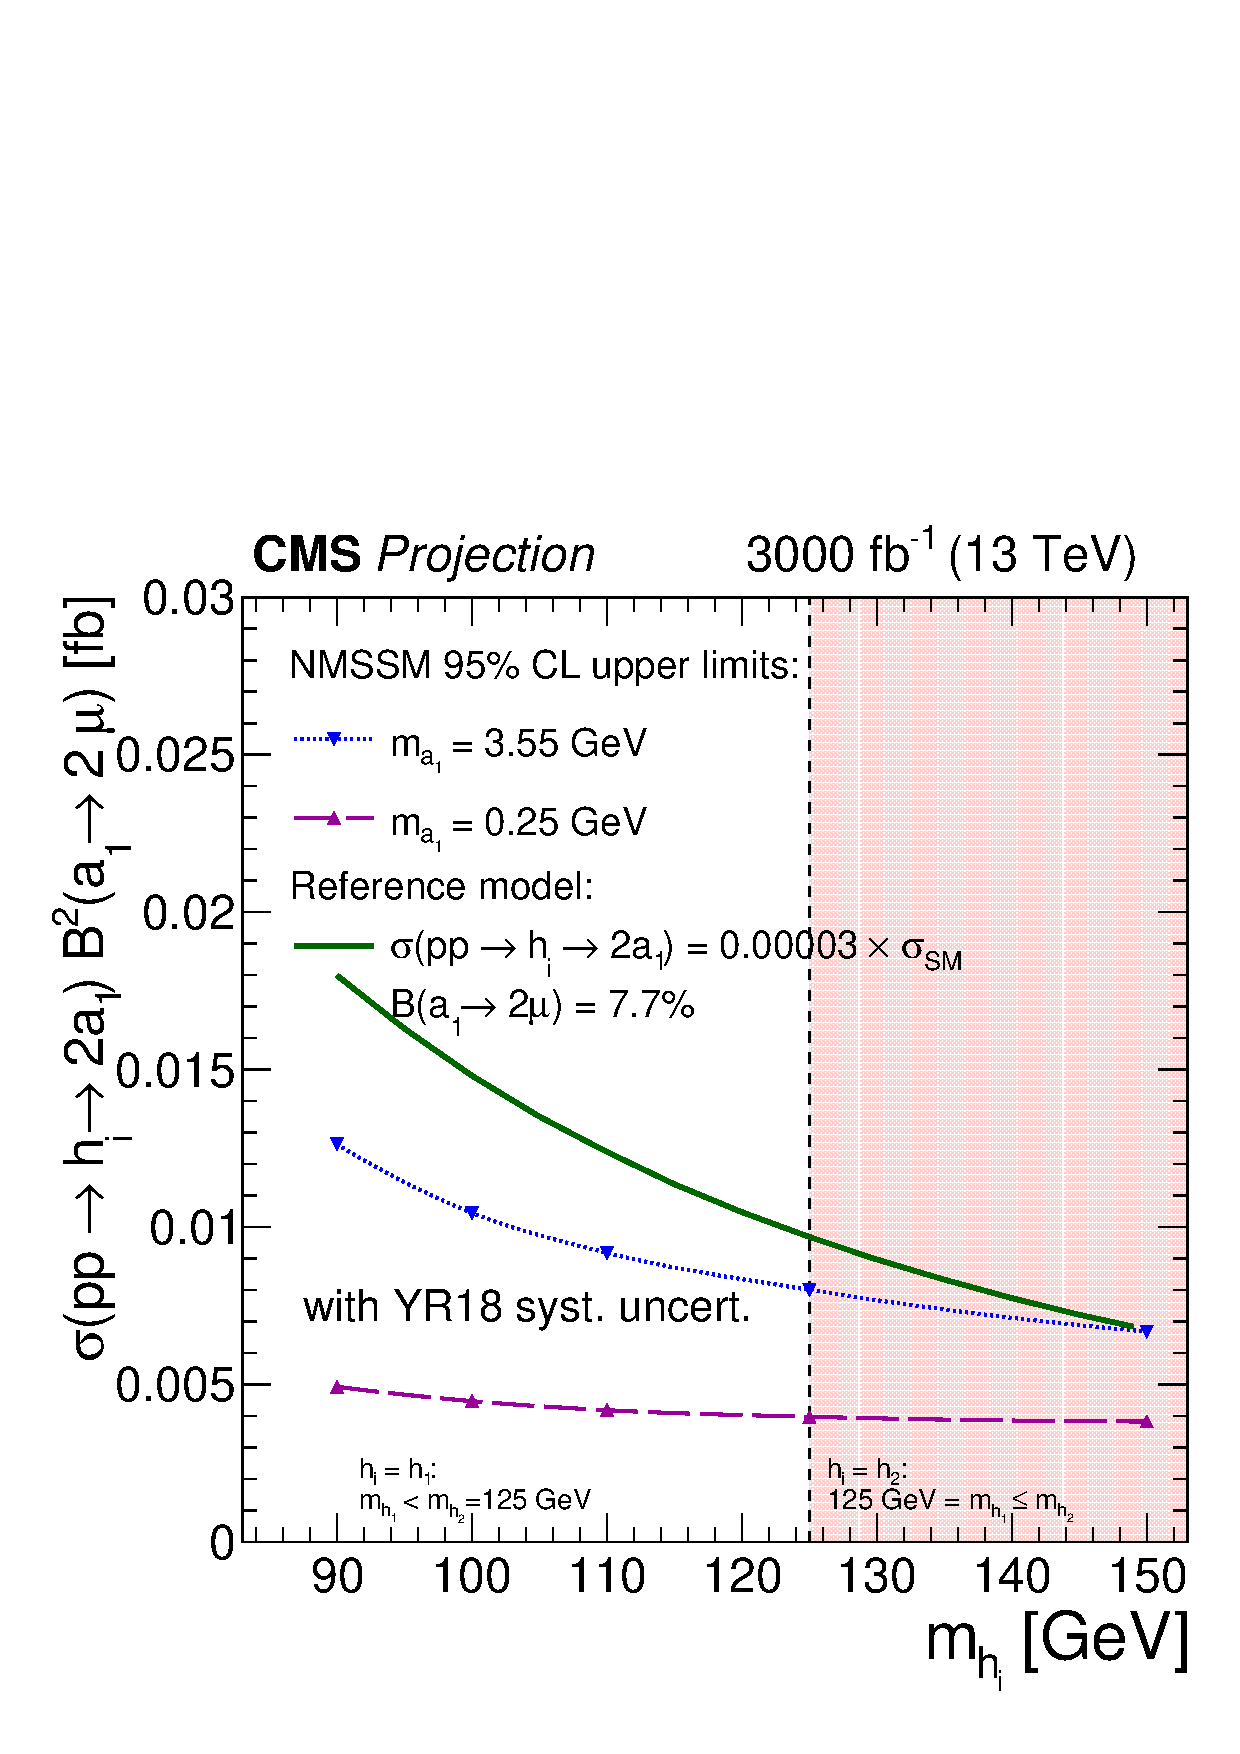
\includegraphics[width=0.5\textwidth]{plots/nmssm_plots_scenario_2/CSxBR_NMSSM_vs_mh_3000.pdf}
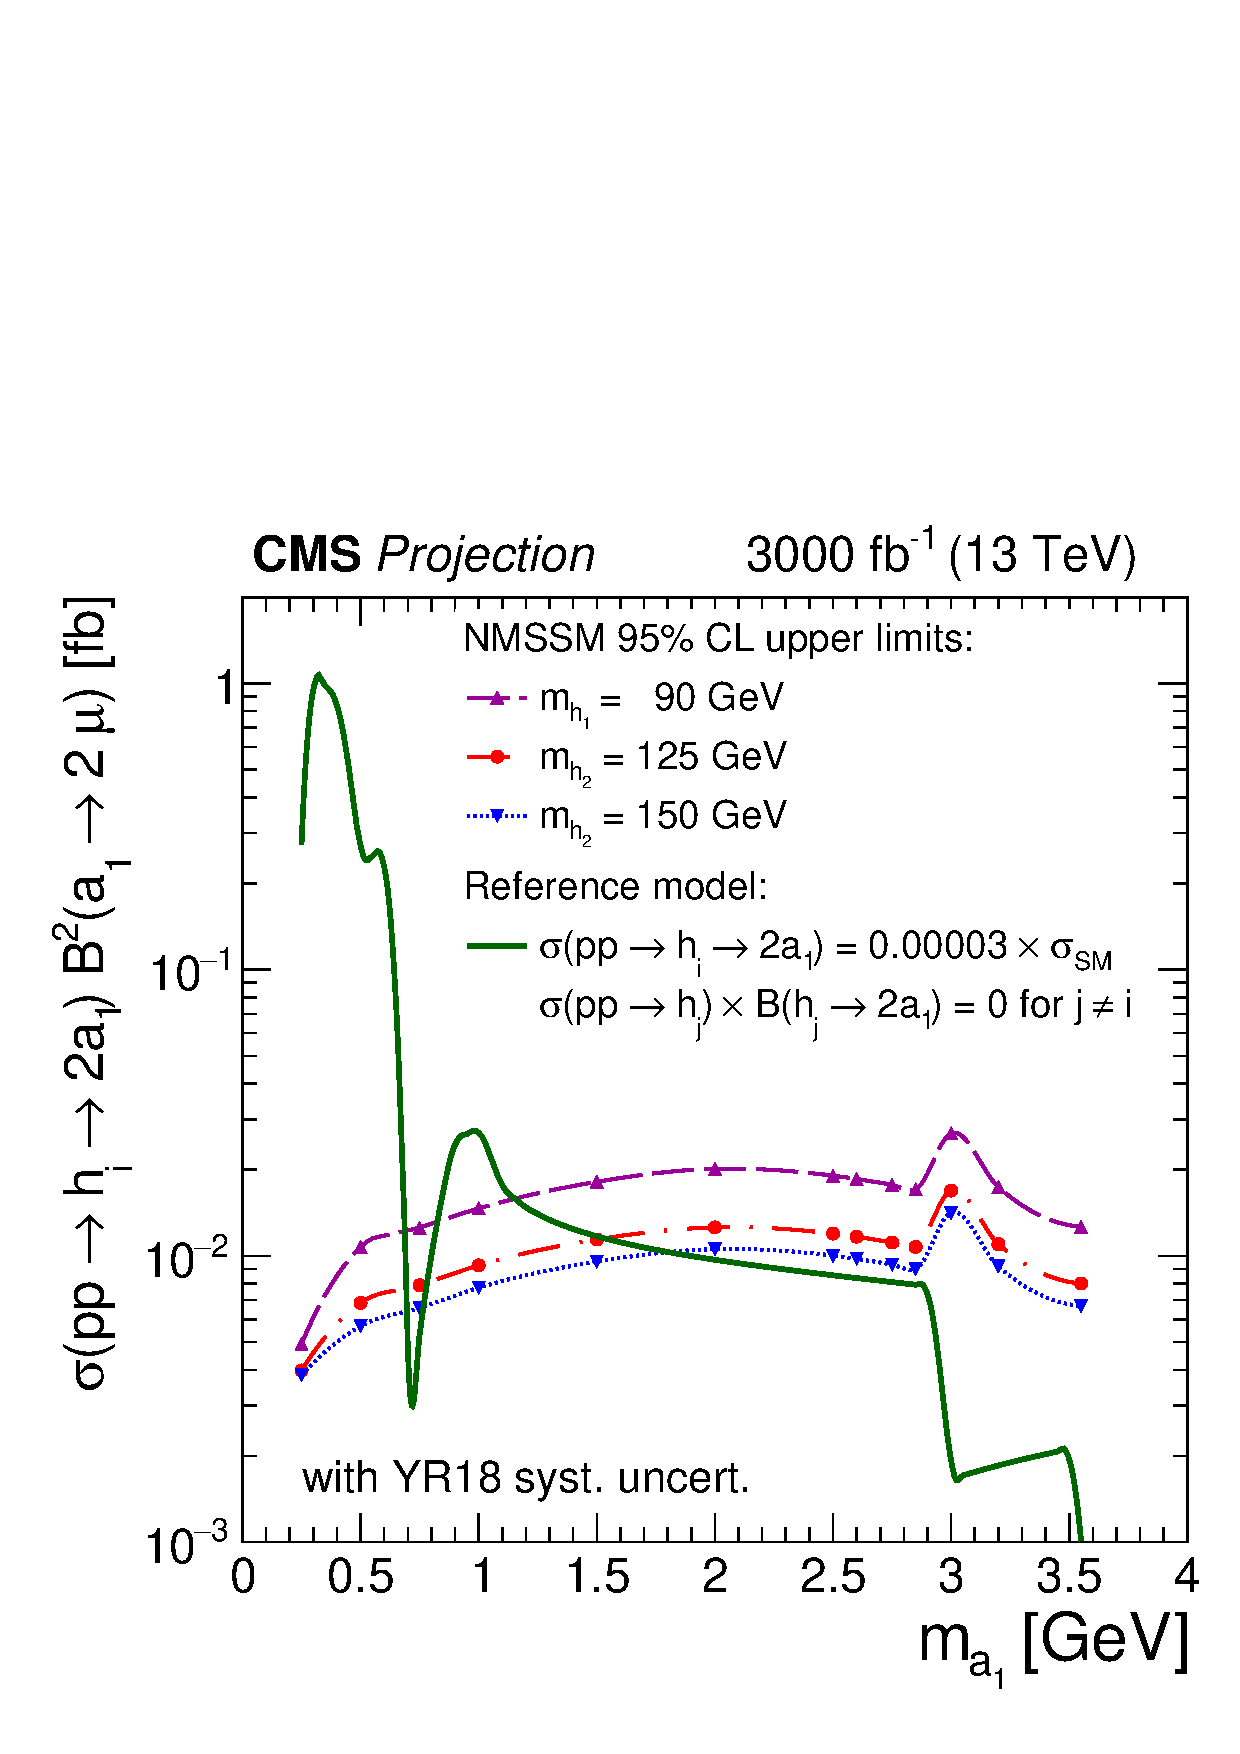
\includegraphics[width=0.5\textwidth, clip, trim=0cm 0cm 0cm 0cm]{plots/nmssm_plots_scenario_2/CSxBR_vs_ma_3000.pdf}
\caption{Left: Projected 95\% \CL upper limits for 3000\fbinv of data in the NMSSM benchmark model as functions of \MPhOneTwo on ${\sigma(\Pp\Pp \to \PhOneTwo \to 2 \PaOne) \mathcal{B}^2(\PaOne \to 2 \PGm)}$ with $\MPaOne=0.25\GeV$ (dashed curve)
and $\MPaOne=3.55\GeV$ (dotted curve).
The limits are compared to a representative predicted rate (solid curve) obtained using a simplified model where
$\sigma (\Pp\Pp \to \PhOne)=\sigma_\mathrm{SM}(\MPhOne)$~\cite{Dittmaier:2011ti},
${\sigma (\Pp\Pp \to \PhTwo) \mathcal{B}(\PhTwo \to 2 \PaOne) = 0}$, $\mathcal{B}(\PhOne \to 2 \PaOne) = 0.3\%$,
and $\mathcal{B}(\PaOne \to 2\PGm) = 7.7\%$. For the chosen $\mathcal{B}(\PaOne \to 2\PGm)$, taken from Ref.~\cite{Dermisek:2010mg}, $\MPhOne = 2\GeV$ and NMSSM parameter $\tanb = 20$. Right: Projected 95\% \CL upper limits for 3000\fbinv of data in the NMSSM benchmark model on $\sigma(\Pp\Pp \to \PhOneTwo \to 2 \PaOne) \mathcal{B}^2(\PaOne \to 2 \PGm)$ with $\MPhOne=90\GeV$ (dashed curve),
$\MPhOne=125\GeV$ (dash-dotted curve), and $\MPhTwo=150\GeV$ (dotted curve). These limits are compared to a representative predicted rate (solid curve) from a simplified case in which $\mathcal{B}(\PhOne \to 2 \PaOne) = 0.3\%$,
$\sigma (\Pp\Pp \to \PhOne)=\sigma_\mathrm{SM}(\MPhOne = 125\GeV)$~\cite{Dittmaier:2011ti}, and
$\sigma (\Pp\Pp \to \PhTwo)  \mathcal{B}(\PhTwo \to 2 \PaOne) = 0$. Additionally, $\mathcal{B}(\PaOne \to 2\PGm)$
as a function of $\MPhOne$ is taken from Ref.~\cite{Dermisek:2010mg} and assumes that the NMSSM parameter \tanb = 20.}
\label{fig:my_label2}
\end{figure}

\begin{figure}
\centering
\includegraphics[width=0.5\textwidth]{plots/darksusy_plots_scenario_2/Limit_DarkPhoton_Epsilon_vs_mass_FTR_scenario2.pdf}%FIXME replace S2
\caption{Projected 95\% \CL upper limits (black solid curves) for 3000\fbinv of data as interpreted in the dark SUSY benchmark model, where the process is $\Pp\Pp \to \Ph \to 2\nOne \to 2\gammaDark+2\nDark \to  4\PGm+\PX$, with $m_{\nOne}=10$\GeV and $\MgammaDark=1$\GeV.
The limits are presented in the plane of the parameters ($\varepsilon$ and \MgammaDark). The colored contours represent different values of $\mathcal{B}(\Ph \to 2\gammaDark + \PX)$ that range from 0.1 to 40\%. }
\label{fig:my_label4}
\end{figure}


